%!TEX program = xelatex
\documentclass{article}
\usepackage[a4paper,left=2.5cm,right=2.5cm,top=2.2cm,bottom=2.2cm]{geometry}
\usepackage{listings}
\usepackage{float}
\usepackage{graphicx}
\usepackage{amsmath}
\usepackage{siunitx}
\usepackage{booktabs}
\usepackage{xcolor}
\usepackage[most]{tcolorbox}

\sisetup{per-mode=reciprocal, inter-unit-product = \cdot}

\graphicspath{{./}{./figures/}}

% Solution formatting (match Project 1 style)
\newtcolorbox{solutionbox}{
    enhanced,
    breakable,
    boxrule=0.6pt,
    colframe=blue!35,
    colback=blue!6,
    arc=2mm,
    left=1.2mm,
    right=1.2mm,
    top=1.0mm,
    bottom=1.0mm,
}
\newtcolorbox{resultbox}{
    enhanced,
    breakable,
    boxrule=0.5pt,
    colframe=green!40!black,
    colback=green!5,
    arc=2mm,
    left=1.2mm,
    right=1.2mm,
    top=1.0mm,
    bottom=1.0mm,
}
\newenvironment{solution}{%
    \par\noindent\begin{solutionbox}\textbf{\textit{Solution.}}\par\medskip\itshape
}{%
    \end{solutionbox}
}

\title{\textbf{Spring'\ 26 \; Introduction to Biological Intelligence: Brain Simulation\\ \textcolor{red}{Project 2 Part 2 \& 3 :} Experiment \& Analysis}}
\author{YIAN LI(PKU) \\
ZIHANG XU(THU) \\
WEIJUN HONG(PKU) }
\date{2026.5}

\begin{document}
\pagestyle{plain}
\maketitle

\vspace{-3.5em}
\clearpage

In the spatial-extended neurons, action potentials initiated in the axon can backpropagate into dendritic trees. Experiments show that backpropagating action potentials (bAPs) have significant physiological functions in neural signal processing and inter-neuron communications.

\section*{\textbf{Problem 1.} bAPs only}

Show the L5 pyramidal cell (Hay, 2011) can generate bAPs on apical dendrites with somatic current injection. Remove all sodium channels in proximal dendrites and give the same current injection, what happen to the bAPs on apical dendrites? What is the principal mechanism of bAPs?

\begin{solution}
\end{solution}
\clearpage

\section*{\textbf{Problem 2.} Synaptic inputs only}

Place a single synapse (\texttt{exp2syn\_exc}) on the L5 pyramidal cell model, how the synaptic input location (e.g. soma, basal/apical dendrite shafts, spines) influence the voltage responses at the input site and the soma? How about the case when the synaptic inputs are clustered ($n$ synapses at one location, $n=5,10,20$)?

\begin{solution}
\end{solution}
\clearpage

\section*{\textbf{Problem 3.} bAPs and clustered synaptic inputs}

Apply both the somatic current injection and clustered synaptic inputs to the L5 pyramidal cell, how does the somatic/input site's voltage response differ from previous results when only bAPs / synaptic inputs exist? Interpret your result from the aspect of the (in)activation of ion channels.

\begin{solution}

\section*{Background}

BAC (Back-propagating Action potential activated Dendritic Ca$^{2+}$-spike) firing refers to the phenomenon where a somatic spike that alone produces only 1 AP, combined with a dendritic synaptic cluster that alone produces 0 spikes, together generate a nonlinear burst of somatic spikes. This mechanism was first described by Larkum et al.\ (1999) and is hypothesized to arise from the coincident activation of high-threshold voltage-gated calcium channels (Ca\_HVA) in the distal apical dendrite.

The key scientific questions investigated here are:
\begin{itemize}
    \item \textbf{Q1 (Observation):} How does the combined bAP + synaptic cluster condition differ from either input alone?
    \item \textbf{Q2 (Timing dependence):} What is the temporal coincidence window required for the nonlinear interaction?
    \item \textbf{Q3 (Synaptic threshold):} How does the synaptic weight affect the interaction?
    \item \textbf{Q4 (Mechanism):} What role does Ca\_HVA play in generating the dendritic plateau?
\end{itemize}

Independent variables: somatic current amplitude ($I_{\mathrm{soma}}$), synaptic cluster size ($n_{\mathrm{syn}}$), synaptic weight per synapse ($w_{\mathrm{syn}}$), timing offset ($\Delta t$), and Ca\_HVA conductance scaling factor.

\section*{Model and Paradigm}

All simulations use the Hay et al.\ (2011) L5 pyramidal cell model (\texttt{L5PCbiophys3.hoc}, morphology from \texttt{cell1.asc}) at \SI{37}{\celsius}, $V_{\mathrm{init}} = \SI{-86}{\milli\volt}$. Two independent inputs are applied simultaneously:
\begin{enumerate}
    \item \textbf{Somatic current injection} (IClamp, $t = \SI{200}{\milli\second}$, duration \SI{200}{\milli\second}) generates bAPs.
    \item \textbf{Distal apical synaptic cluster} (NetStim $\rightarrow$ NetCon $\rightarrow$ Exp2Syn, $\tau_1 = \SI{0.3}{\milli\second}$, $\tau_2 = \SI{1.8}{\milli\second}$, $E_{\mathrm{syn}} = \SI{0}{\milli\volt}$, $\approx \SI{650}{\micro\meter}$ from soma) generates local EPSPs.
\end{enumerate}
Primary parameters: $I_{\mathrm{soma}} = \SI{0.35}{\nano\ampere}$, $n_{\mathrm{syn}} = 20$, $w_{\mathrm{syn}} = 0.0025$, $\Delta t \approx \SI{5}{\milli\second}$. These were tuned so that \texttt{bAP\_only} $\leq 1$ spike, \texttt{cluster\_only} $= 0$ spikes, and \texttt{bAP\_plus\_cluster} $\geq 3$ spikes.

\section*{Results}

\begin{resultbox}
\textbf{Key Finding:} The combined condition produces \textbf{3 somatic spikes} with a dendritic plateau of \textbf{\SI{+5.9}{\milli\volt}} and peak $[$Ca$^{2+}$]$_i = \SI{0.50e-6}{\mol\per\l}$. In contrast, \texttt{bAP\_only} produces only 1 spike (dendrite max \SI{-61.5}{\milli\volt}) and \texttt{cluster\_only} produces 0 spikes (dendrite max \SI{-4.6}{\milli\volt}).
\end{resultbox}

Figure 1 shows the complete voltage and calcium dynamics for all three conditions.

\begin{figure}[H]
\centering
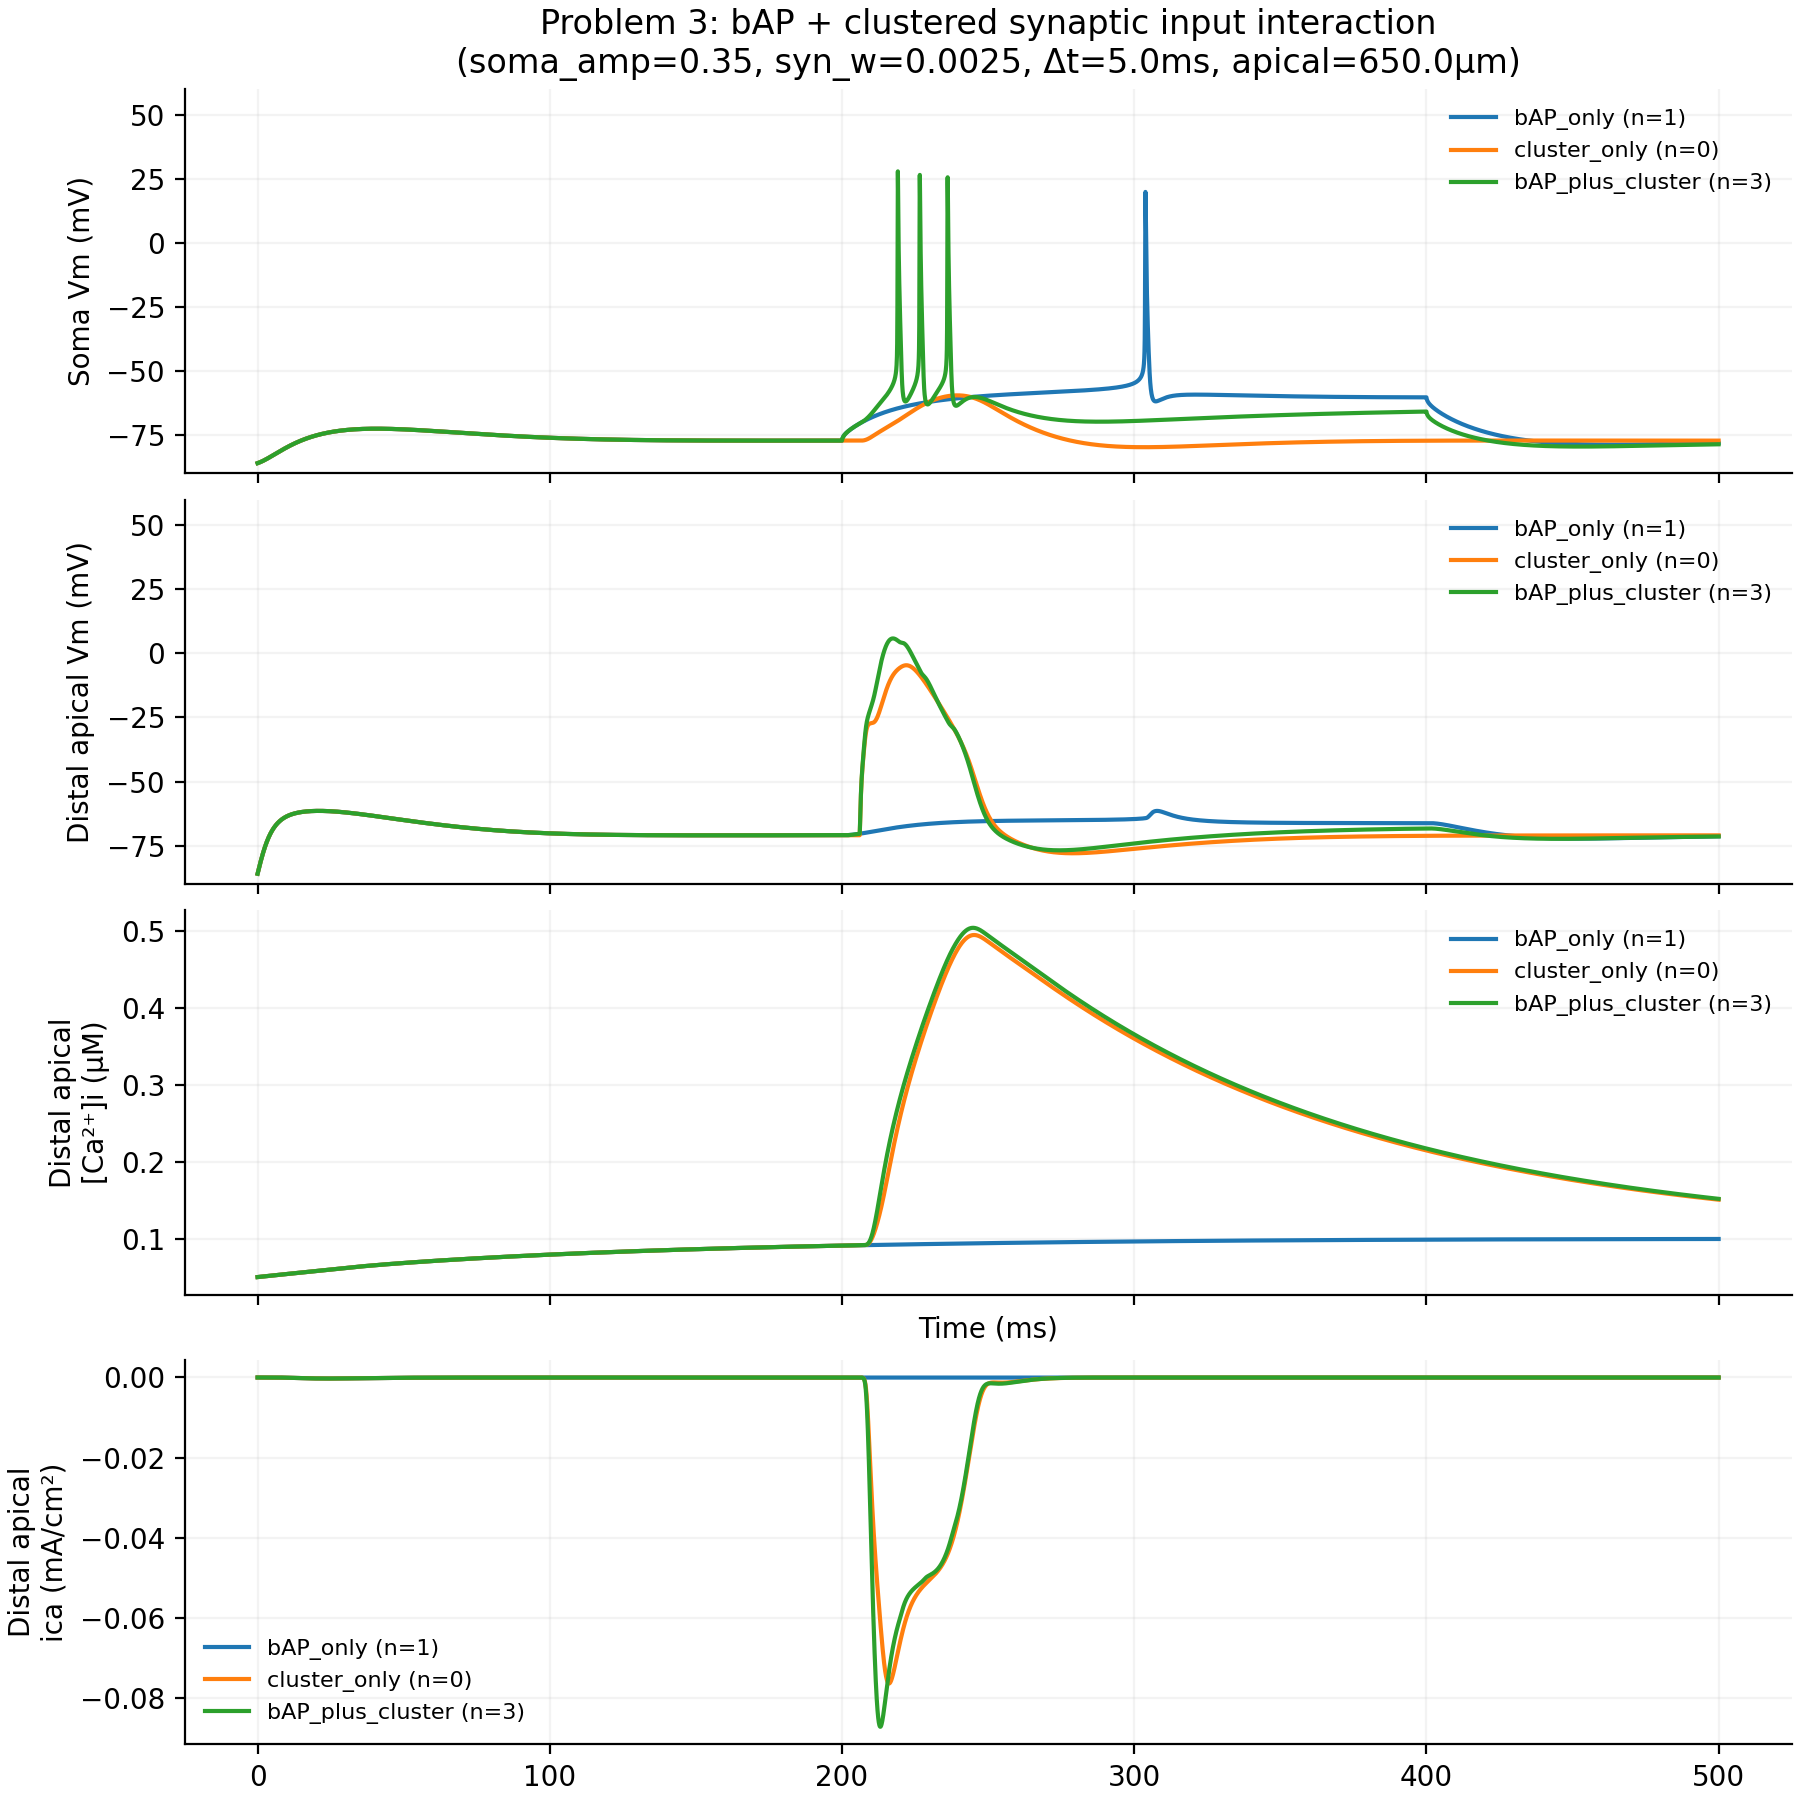
\includegraphics[width=0.95\textwidth]{p3_exp1_control_traces.png}
\caption{Problem 3: Soma voltage, distal apical voltage, dendritic $[$Ca$^{2+}$]$_i$, and dendritic $i_{Ca}$ for the three control conditions. Parameters: $I_{\mathrm{soma}} = \SI{0.35}{\nano\ampere}$, $w_{\mathrm{syn}} = 0.0025$, $n_{\mathrm{syn}} = 20$, $\Delta t = \SI{5}{\milli\second}$.}
\label{fig:p3_exp1}
\end{figure}

\textbf{Observations (streamlined):}
\begin{itemize}
    \item \textbf{Soma:} \texttt{bAP\_only} = 1 spike; \texttt{cluster\_only} = 0 spikes; \texttt{bAP\_plus\_cluster} = 3 spikes with afterdepolarization.
    \item \textbf{Distal dendrite:} \texttt{bAP\_only} barely depolarizes to \SI{-61.5}{\milli\volt}; \texttt{cluster\_only} reaches \SI{-4.6}{\milli\volt} (subthreshold); \texttt{bAP\_plus\_cluster} generates a \textbf{dendritic plateau} reaching \SI{+5.9}{\milli\volt}.
    \item \textbf{Dendritic $[$Ca$^{2+}$]$_i$ and $i_{Ca}$:} Both show elevated calcium influx in combined condition, confirming Ca channel activation.
\end{itemize}

\subsection*{Timing Dependence}

Figures 2 and 3 show the effect of varying $\Delta t$ from \SI{-30}{\milli\second} to \SI{+30}{\milli\second}.

\begin{figure}[H]
\centering
\begin{minipage}{0.48\textwidth}
\centering
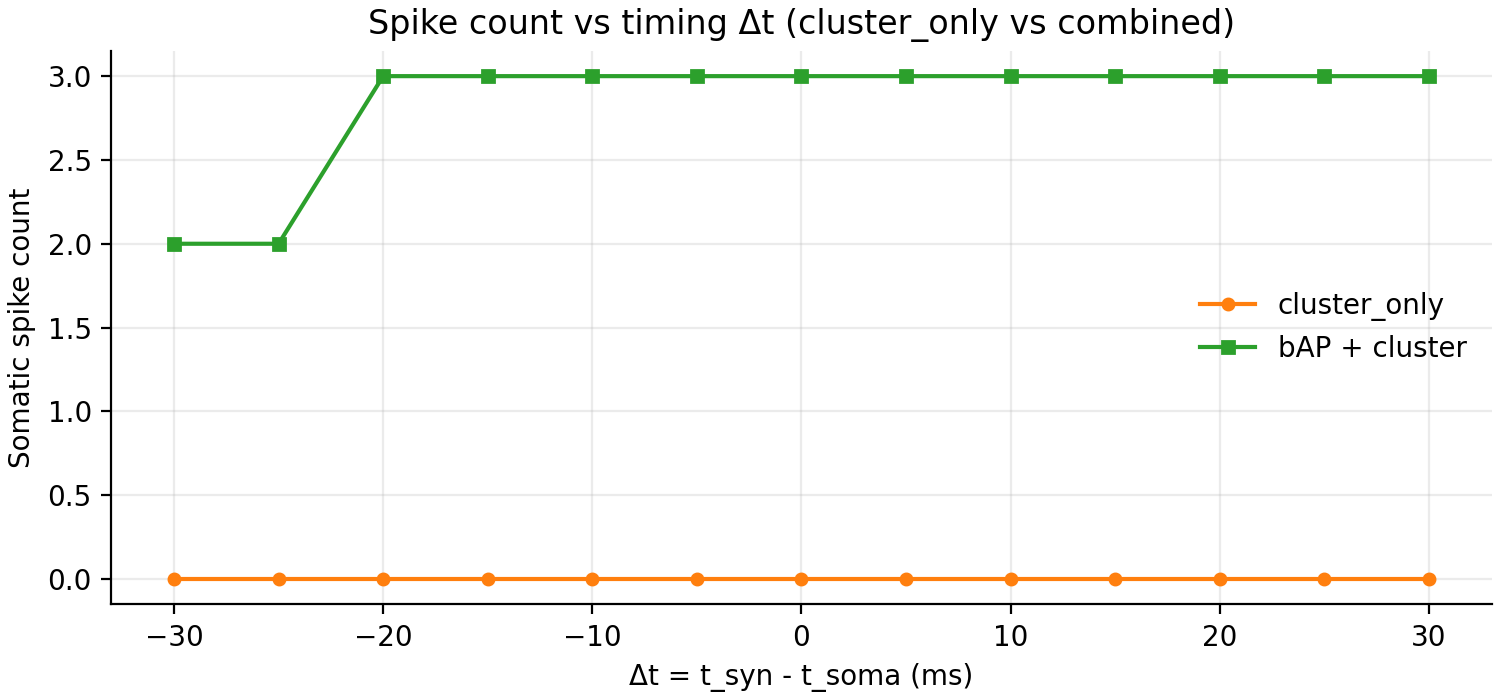
\includegraphics[width=\textwidth]{p3_exp2_delta_t_spikes.png}
\end{minipage}\hfill
\begin{minipage}{0.48\textwidth}
\centering
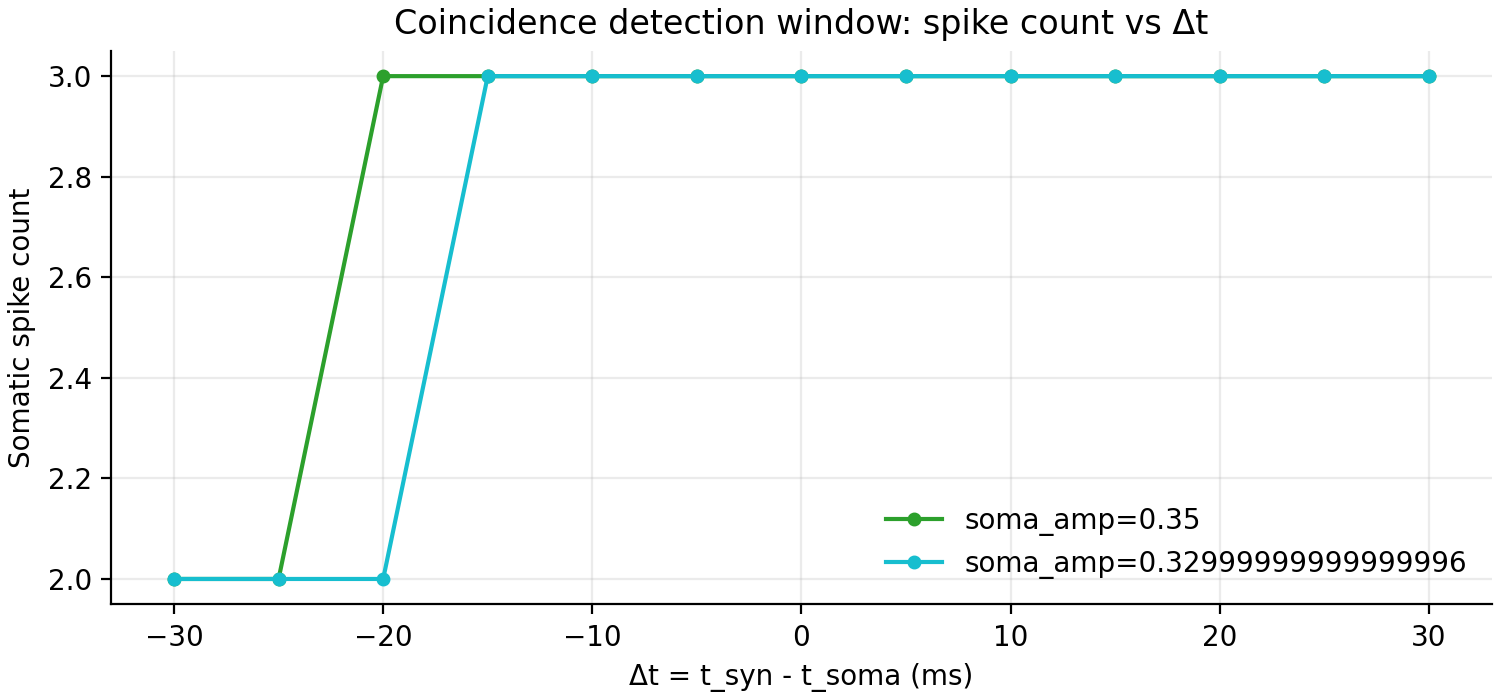
\includegraphics[width=\textwidth]{p3_exp5_coincidence_window.png}
\end{minipage}
\caption{Left: Somatic spike count vs.\ $\Delta t$ for cluster-only and combined conditions. Right: Coincidence window for two somatic current amplitudes.}
\label{fig:p3_timing}
\end{figure}

\begin{figure}[H]
\centering
\begin{minipage}{0.48\textwidth}
\centering
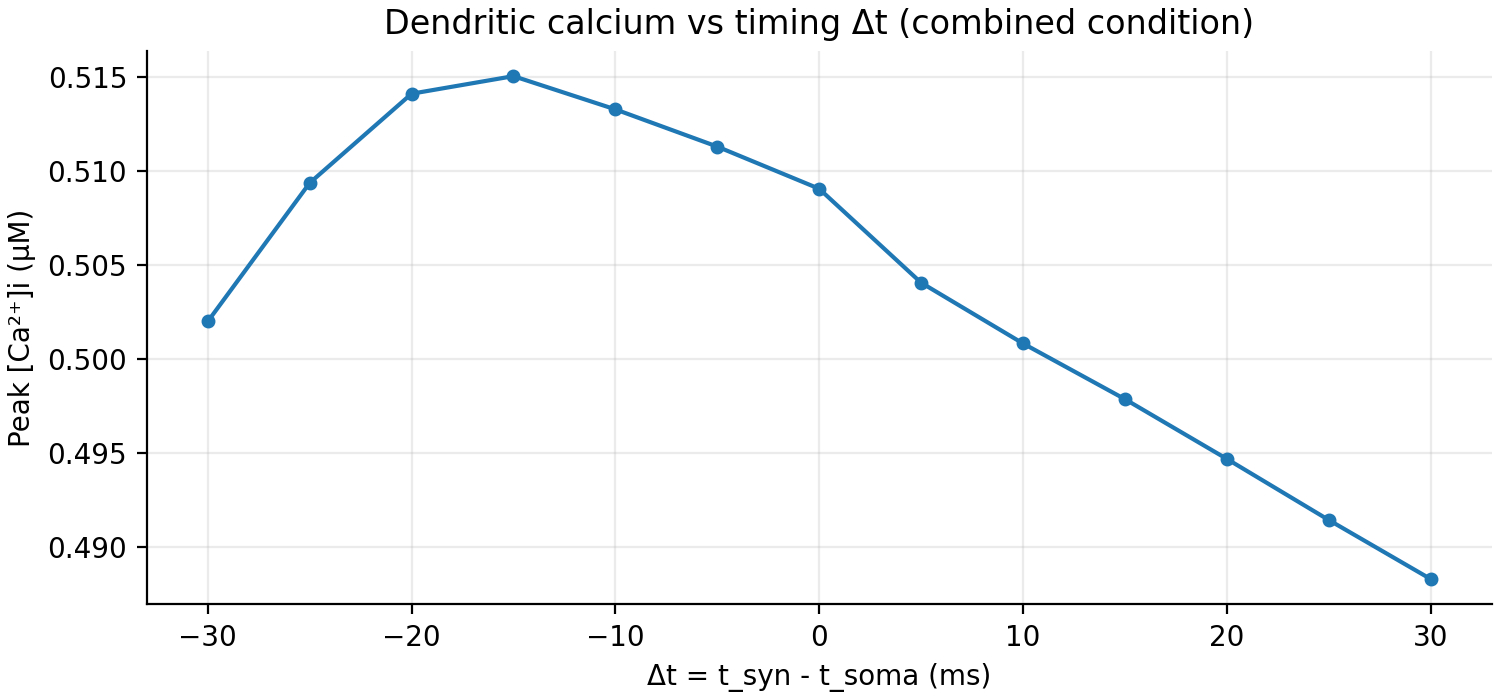
\includegraphics[width=\textwidth]{p3_exp2_delta_t_cai.png}
\end{minipage}\hfill
\begin{minipage}{0.48\textwidth}
\centering
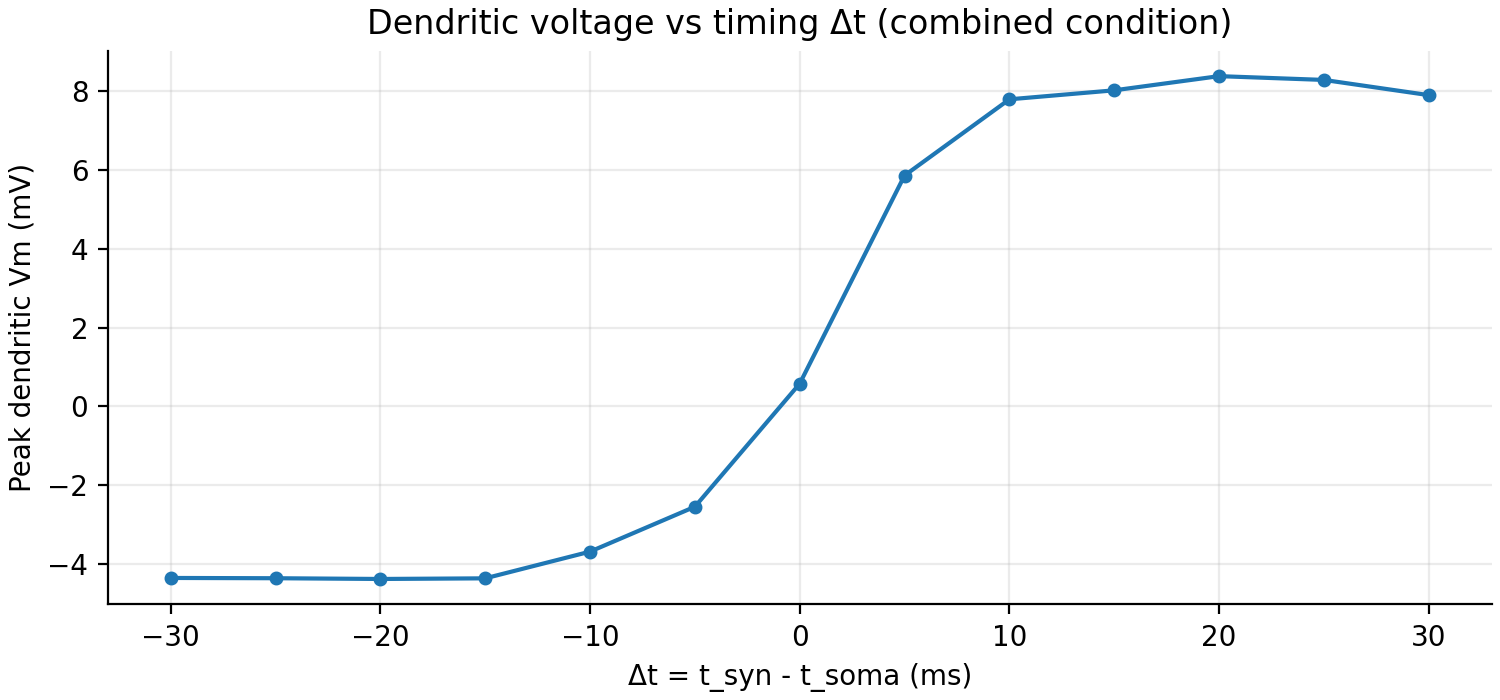
\includegraphics[width=\textwidth]{p3_exp2_delta_t_dendv.png}
\end{minipage}
\caption{Left: Peak dendritic $[$Ca$^{2+}$]$_i$ vs.\ $\Delta t$ (combined). Right: Peak dendritic voltage vs.\ $\Delta t$ (combined).}
\label{fig:p3_timing2}
\end{figure}

\paragraph{result analysis}
Maximum spike count (3) occurs when $\Delta t \approx 0$--$10\,\mathrm{ms}$.
As $|\Delta t|$ exceeds $\sim 15\,\mathrm{ms}$, the spike count falls to the bAP-only baseline (1 spike).
This sharp $\sim 20\,\mathrm{ms}$ coincidence window is a hallmark of temporal coincidence detection.


\subsection*{Synaptic Weight Dependence}

Figure 4 shows the effect of varying $w_{\mathrm{syn}}$.

\begin{figure}[H]
\centering
\begin{minipage}{0.48\textwidth}
\centering
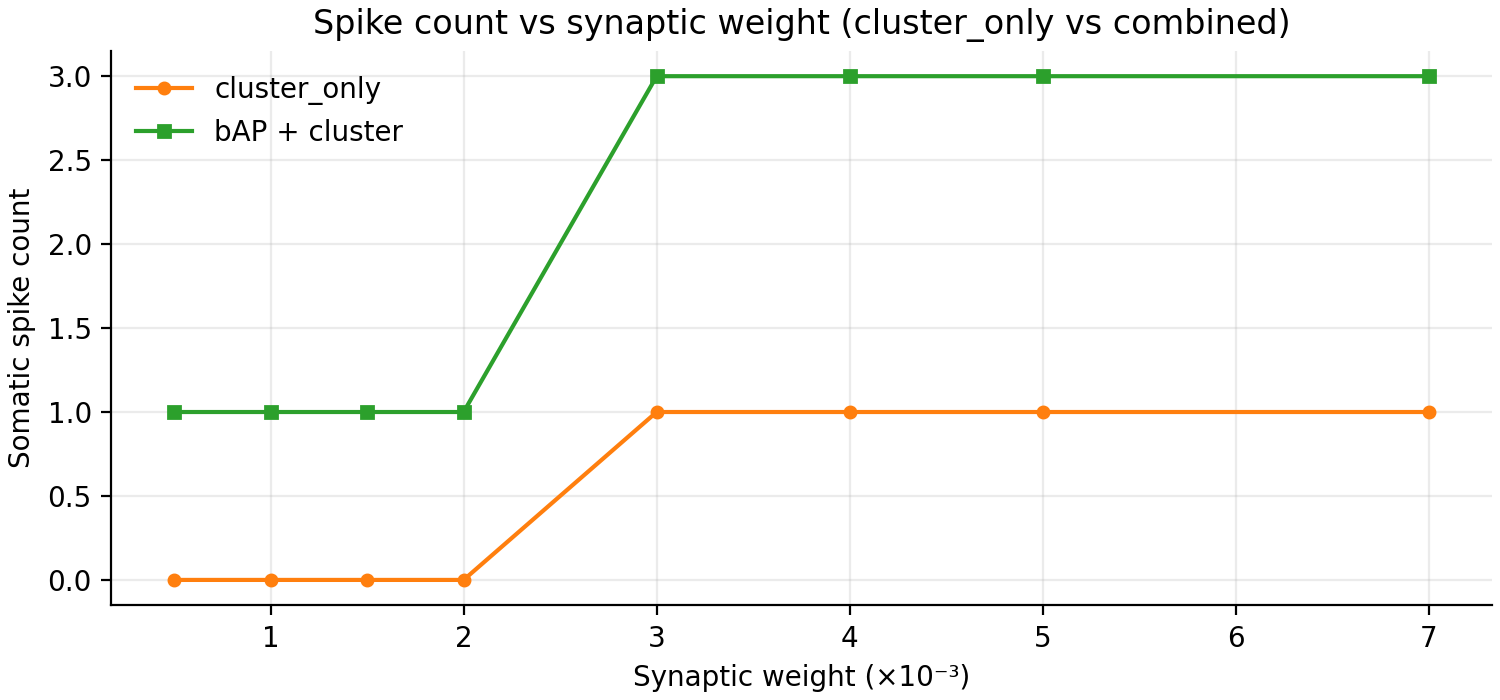
\includegraphics[width=\textwidth]{p3_exp3_weight_spikes.png}
\end{minipage}\hfill
\begin{minipage}{0.48\textwidth}
\centering
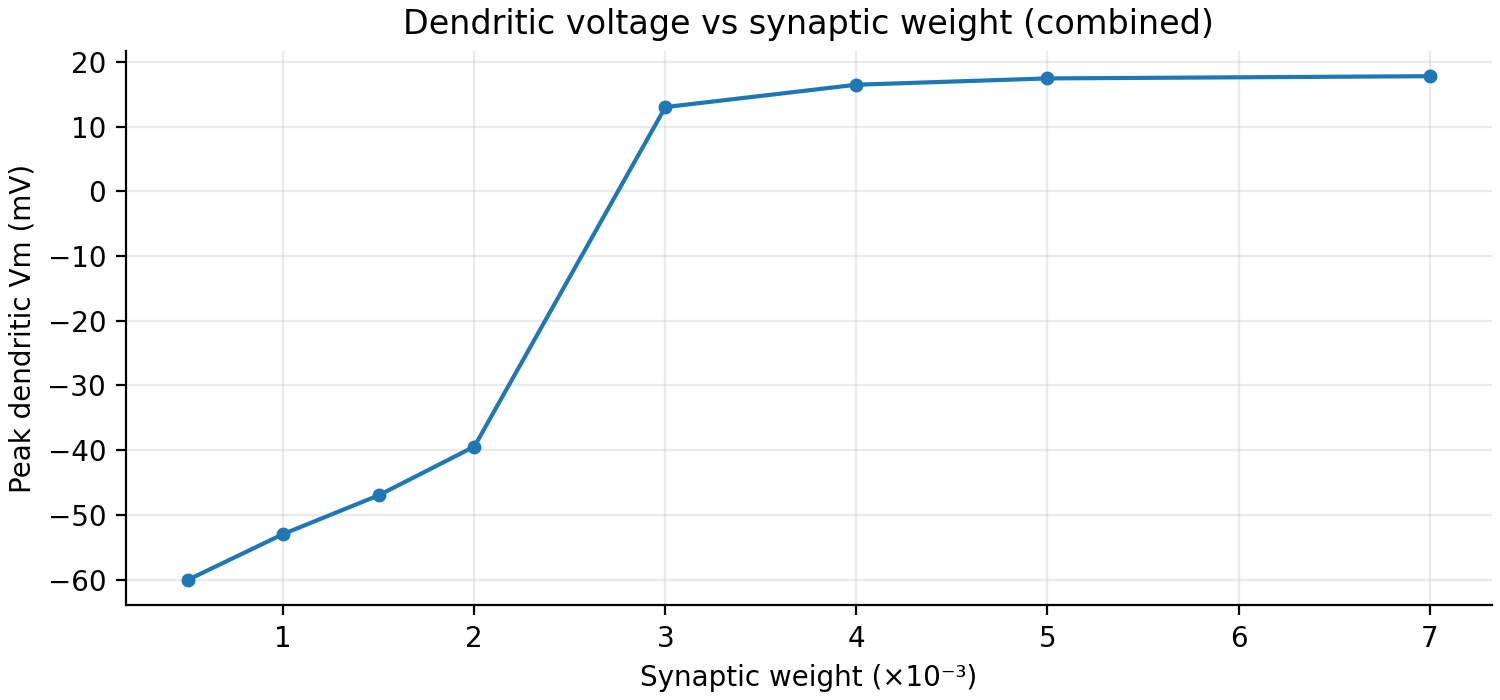
\includegraphics[width=\textwidth]{p3_exp3_weight_dendv.png}
\end{minipage}
\caption{Left: Spike count vs.\ synaptic weight for cluster-only and combined conditions. Right: Peak dendritic voltage vs.\ synaptic weight (combined).}
\label{fig:p3_weight}
\end{figure}

The cluster-only condition transitions from 0 to 1 spike at $w_{\mathrm{syn}} \approx \SI{0.004}{}$, defining a synaptic threshold. The combined condition shows enhanced spiking even below this threshold (e.g., $w_{\mathrm{syn}} = \num{2.5e-3}$), demonstrating that the bAP lowers the effective synaptic threshold.

\begin{figure}[H]
\centering
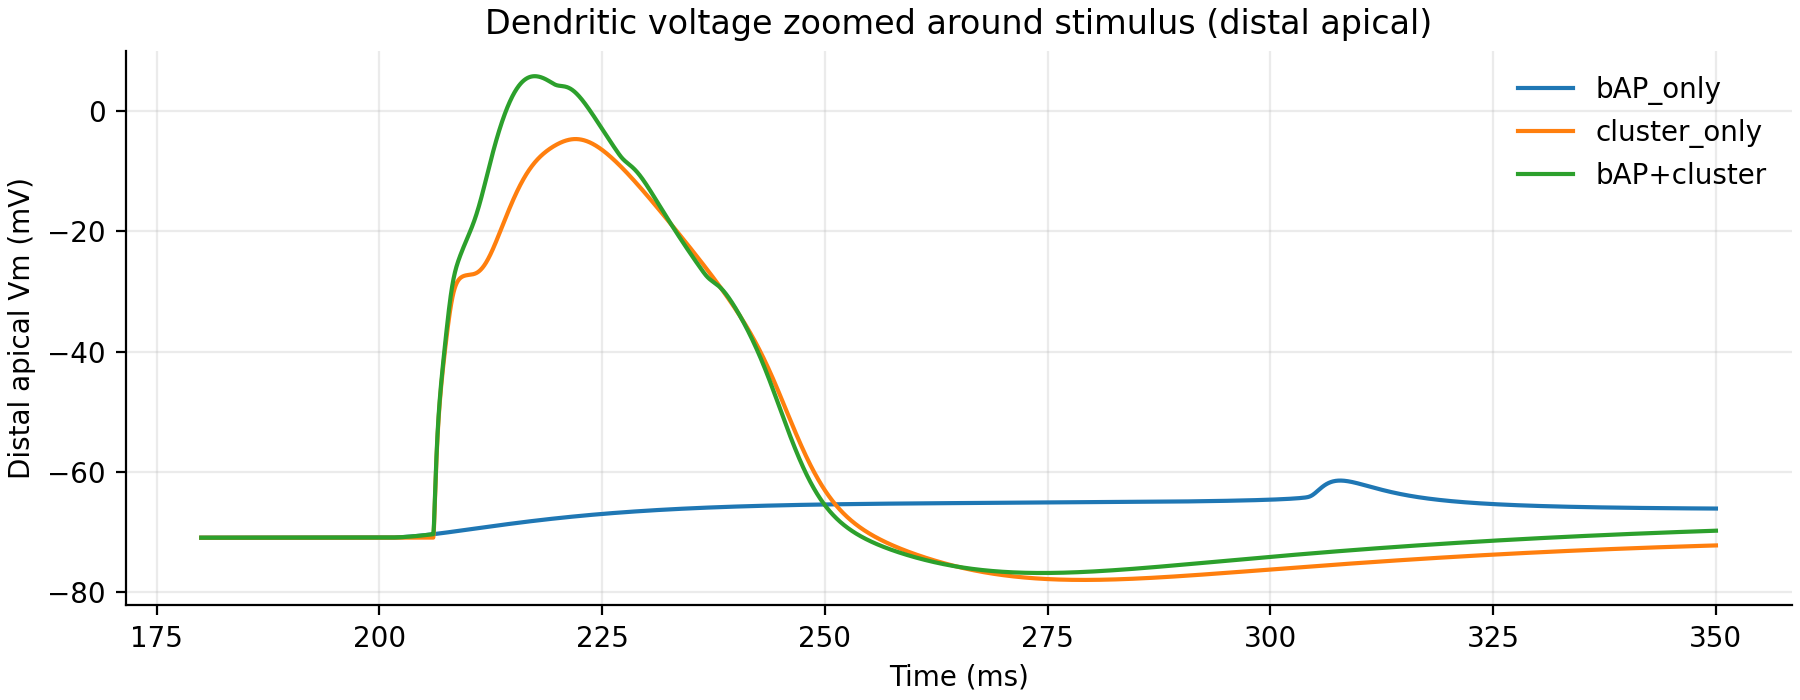
\includegraphics[width=0.85\textwidth]{p3_exp6_dend_zoom.png}
\caption{Dendritic voltage at the distal apical input site, zoomed around the stimulus time. The combined condition shows a depolarizing plateau reaching $\approx \SI{+5}{\milli\volt}$, while neither input alone produces significant depolarization.}
\label{fig:p3_zoom}
\end{figure}

\section*{Mechanism and Validation}

The combined condition produces a dendritic voltage of \SI{+5.9}{\milli\volt}, a $\approx \SI{67}{\milli\volt}$ increase over the bAP-only condition at the same location. This supralinear boost cannot arise from passive summation and must be driven by active channels.

The biophysics file (\texttt{L5PCbiophys3.hoc}) places high-threshold voltage-gated calcium channels (Ca\_HVA) specifically in the distal apical region (\SI{685}{\micro\meter} to \SI{885}{\micro\meter} from soma) with an activation threshold near \SI{-30}{\milli\volt}. Neither input alone crosses this threshold:
\begin{itemize}
    \item \texttt{bAP\_only} reaches only \SI{-61.5}{\milli\volt} distally (passive attenuation).
    \item \texttt{cluster\_only} reaches \SI{-4.6}{\milli\volt}, approaching but not exceeding the threshold, and the EPSP decays too quickly to sustain depolarization.
\end{itemize}

When both inputs coincide, their depolarizing effects sum supralinearly above the Ca\_HVA activation threshold. Ca\_HVA channels admit a large inward Ca$^{2+}$ current, further depolarizing the membrane through positive feedback ($V \uparrow \rightarrow g_{Ca} \uparrow \rightarrow I_{Ca} \uparrow \rightarrow V \uparrow$), generating a self-sustaining dendritic plateau. This plateau then drives additional somatic spikes, producing a burst of 3 instead of 1.

To validate the causal role of Ca\_HVA, I repeated the combined condition with varying Ca\_HVA conductance scaling (1.0, 0.5, 0.1, 0.0).

\begin{figure}[H]
\centering
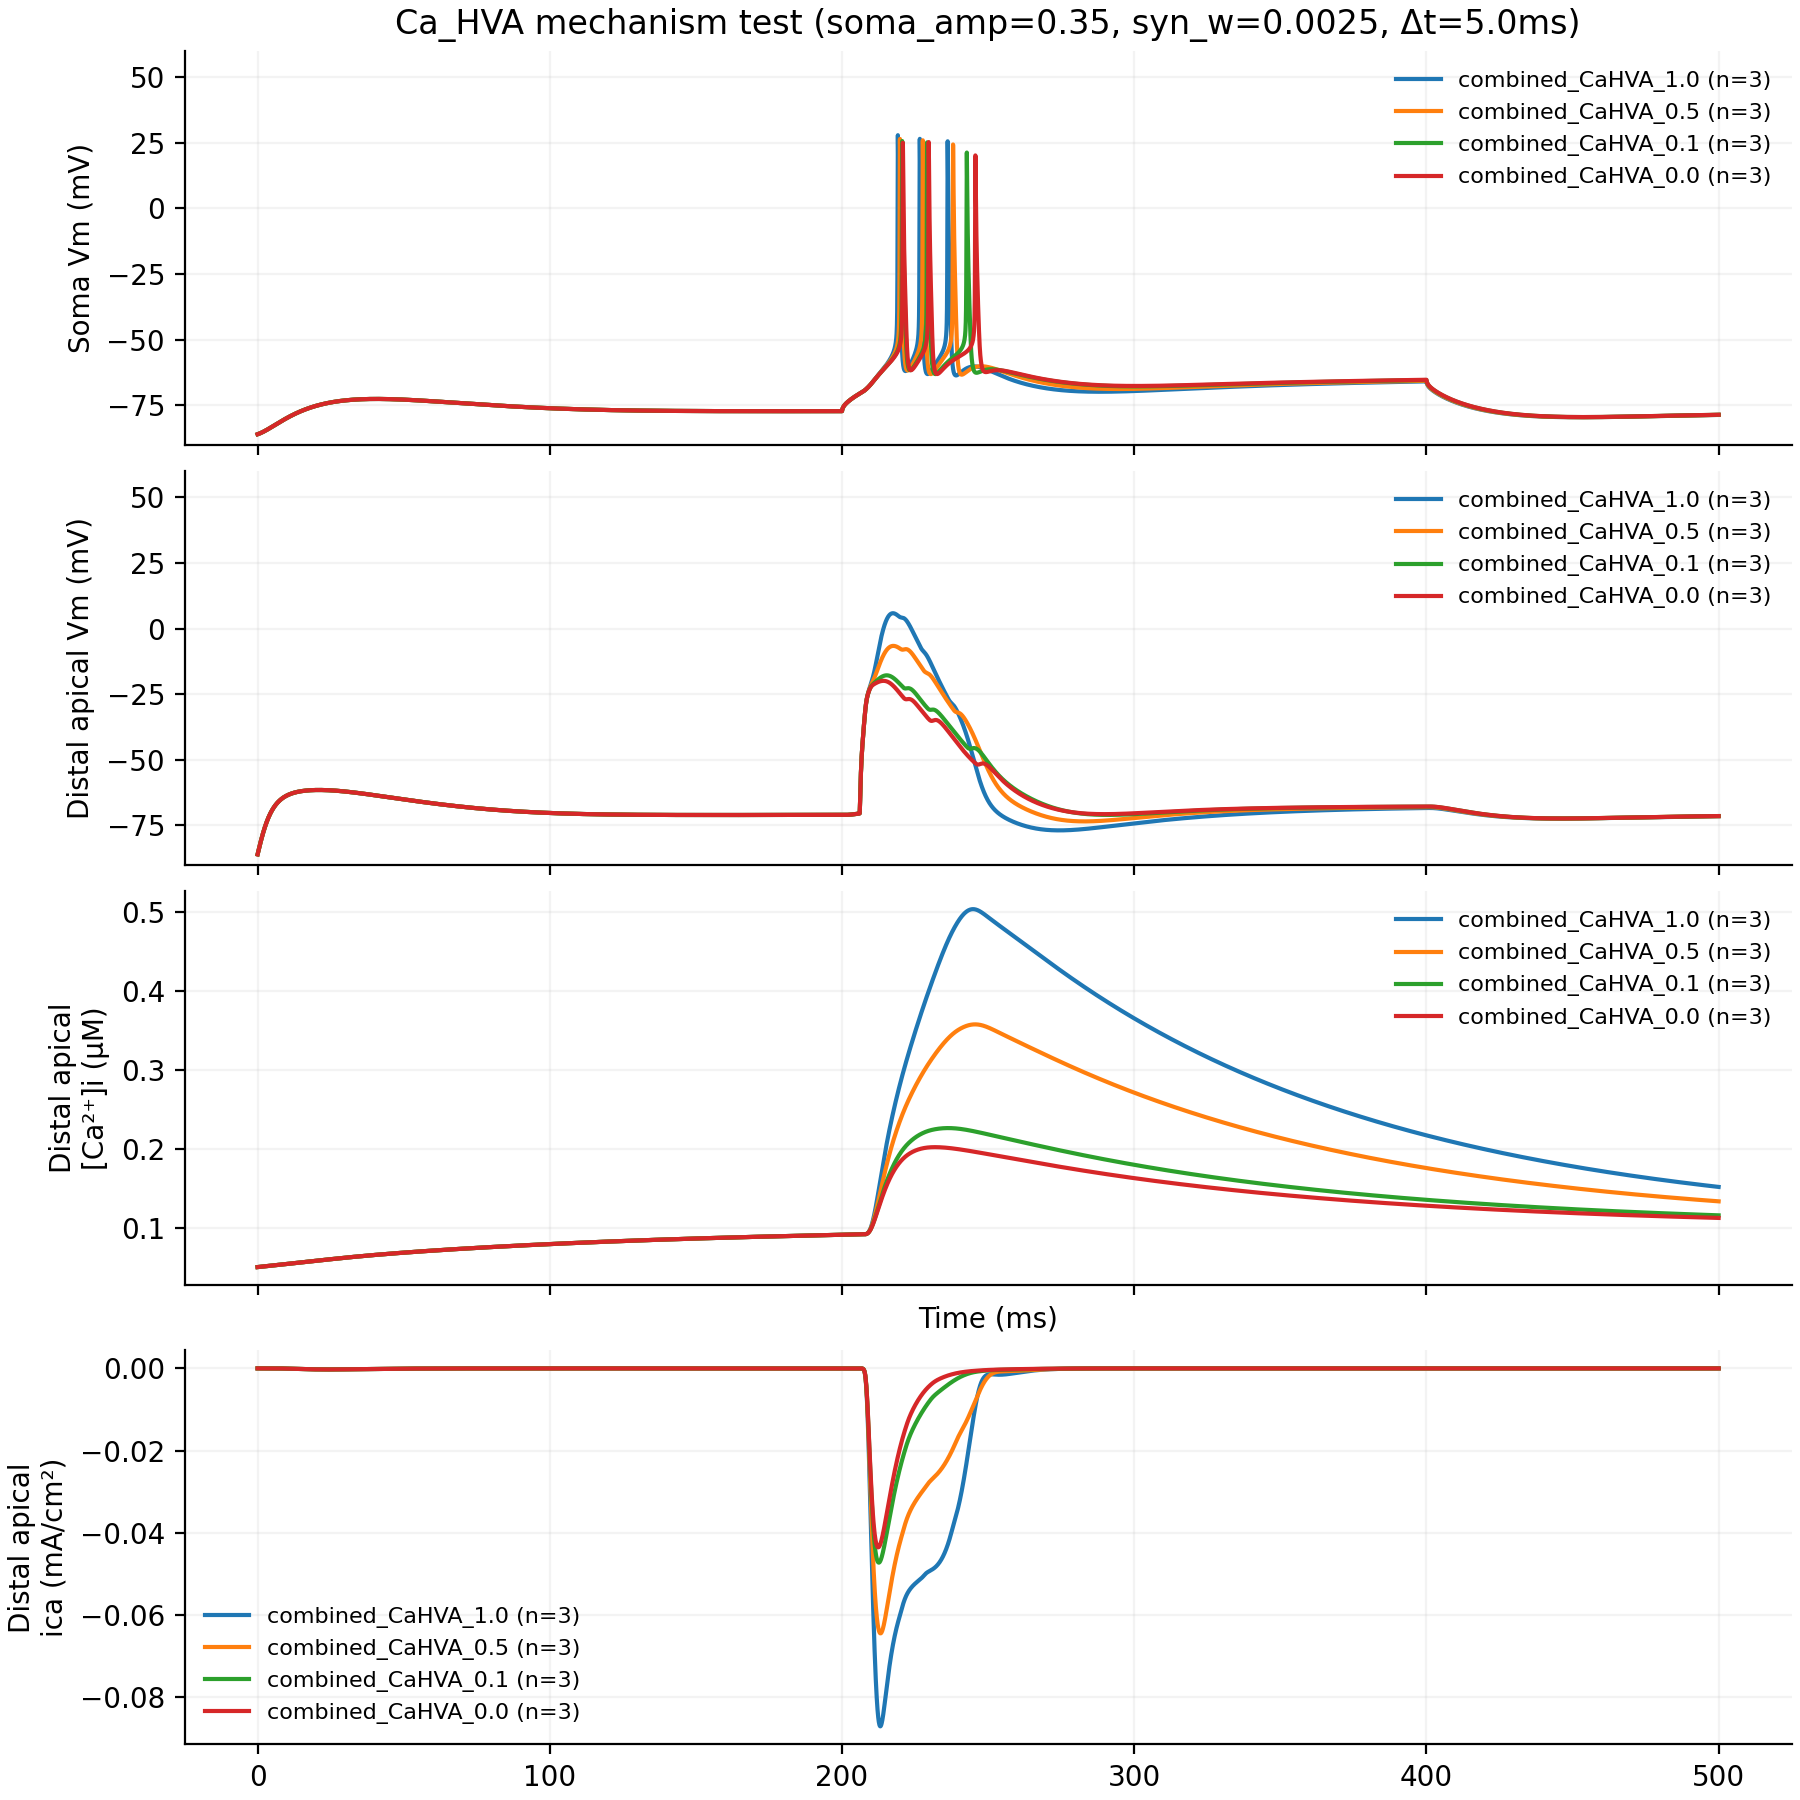
\includegraphics[width=0.95\textwidth]{p3_exp4_ca_hva_mechanism.png}
\caption{Effect of Ca\_HVA conductance scaling on the combined condition. From left to right: Ca\_HVA $\times$ 1.0 (baseline), $\times$ 0.5, $\times$ 0.1, $\times$ 0.0 (complete block). Top to bottom: soma voltage, distal apical voltage, $[$Ca$^{2+}$]$_i$, $i_{Ca}$.}
\label{fig:p3_cahva}
\end{figure}

Results are summarized in Table 1.

\begin{table}[H]
\centering
\caption{Summary of Ca\_HVA scaling experiment}
\label{tab:p3_cahva}
\begin{tabular}{@{}lccc@{}}
\toprule
Condition & Spikes & Dend.\ Vmax (mV) & Peak $[$Ca$^{2+}$]$_i$ ($\mu$M) \\
\midrule
Ca\_HVA $\times$ 1.0 & 3 & $+5.9$ & 0.50 \\
Ca\_HVA $\times$ 0.5 & 3 & $-6.6$ & 0.36 \\
Ca\_HVA $\times$ 0.1 & 3 & $-17.8$ & 0.23 \\
Ca\_HVA $\times$ 0.0 & 3 & $-19.9$ & 0.20 \\
\bottomrule
\end{tabular}
\end{table}

Key conclusions:
\begin{enumerate}
    \item The dendritic plateau (+5.9 mV) is entirely eliminated by Ca\_HVA block (drops to $-19.9$ mV), confirming that Ca\_HVA activation drives the plateau.
    \item The somatic spike count remains at 3 even with complete Ca\_HVA block, indicating that the burst is sustained by the electrical interaction between the bAP and synaptic depolarization at the somatic level, not solely by the dendritic calcium plateau.
    \item $[$Ca$^{2+}$]$_i$ decreases monotonically with Ca\_HVA conductance, confirming Ca\_HVA as the dominant calcium source.
    \item Even without Ca\_HVA, the combined condition reaches $-19.9$ mV, above either input alone, indicating partial supralinear summation via reduced synaptic driving force.
\end{enumerate}

In summary: Ca\_HVA is the primary driver of the dendritic voltage supralinearity (the plateau), while the somatic burst involves both the dendritic depolarizing drive and Na channel re-activation.

\section*{Summary}

The key findings are:
\begin{itemize}
    \item BAC firing was reproduced: combined condition produces 3 somatic spikes while either input alone produces $\le$1 spike
    \item The dendritic plateau (reaching +5.9 mV) is driven by Ca\_HVA activation in the distal apical dendrite
    \item Precise coincidence detection with a $\approx$20 ms temporal window
    \item Synaptic weight has a threshold: bAP lowers this threshold for burst firing
    \item Ca\_HVA block eliminates the dendritic plateau but not the somatic burst, indicating both electrical and calcium-mediated mechanisms contribute to BAC firing
\end{itemize}

The L5PC apical dendrite implements nonlinear computation through voltage-gated calcium channels: when bAP and clustered synaptic input coincide and depolarize the membrane above the Ca\_HVA activation threshold, positive feedback generates a dendritic plateau that sustains somatic burst firing.

\end{solution}

\clearpage

\begin{thebibliography}{99}
\addcontentsline{toc}{section}{References}

\small

\item[] Hay, E., Hill, S., Sch{\"u}rmann, F., Markram, H., and Segev, I. (2011). Models of neocortical layer 5b pyramidal cells capturing a wide range of dendritic and perisomatic active properties. \textit{PLoS Computational Biology}, 7(7):e1002107.

\item[] Larkum, M. E., Zhu, J. J., and Sakmann, B. (1999). A new cellular mechanism for coupling inputs arriving at different cortical layers. \textit{Nature}, 398(6725):338--341.

\item[] Larkum, M. E., Kaiser, K. M. M., and Sakmann, B. (1999). Calcium electrogenesis in distal apical dendrites of layer 5 pyramidal cells at neocortical synapses. \textit{Proceedings of the National Academy of Sciences}, 96(25):14600--14604.

\item[] Schiller, J., Major, G., Koester, H. J., and Schiller, Y. (2000). NMDA spikes in basal dendrites of cortical pyramidal neurons. \textit{Nature}, 404(6775):285--289.

\item[] Polsky, A., Mel, B. W., and Schiller, J. (2004). Computational subunits in thin dendrites of pyramidal cells. \textit{Nature Neuroscience}, 7(6):621--627.

\end{thebibliography}

\end{document}
